\newpage \ \thispagestyle{empty} \newpage

\chapter{Motivazioni alla base del tirocinio}
\label{cap:motivazioni-tirocinio}
Questo capitolo si occupa di definire le motivazioni che hanno portato al compimento del percorso di tirocinio curricolare, dal punto di vista aziendale (si propone quella che, a mio parere, è la visione di \textit{\textbf{Trizeta}}) e dal mio punto di vista,
descrivendo i vincoli, gli obiettivi e le esigenze che il progetto proposto punta a soddisfare.

\section{Strategia aziendale}

% In questa sezione descriverò il rapporto che l'azienda ha nei confronti dei tirocini (universitari e non) dal punto di vista delle tecnologie, dei prodotti, del mercato e dal punto di vista di investimento sulle risorse umane.
In base a quanto ho potuto osservare e capire durante il periodo di \textit{stage}, la strategia di gestione dei tirocini curricolari dell'azienda ospitante persegue i seguenti obiettivi:
\begin{itemize}
    \item \glslink{innovazione}{Innovazione}: come riportato al termine della sezione \hyperref[sec:innovazione]{1.4}, l'introduzione di miglioramenti e novità negli strumenti e nelle tecnologie utilizzate (motivata da esigenze produttive o di mercato)
    può avvalersi (come nel mio caso) del parere motivato del tirocinante, tenendo conto del grado di maturità e delle caratteristiche del lavoro svolto per \textit{testare} le novità da introdurre;
    \item \textbf{Integrazione di prodotti esistenti}: il parco \textit{software \textbf{Trizeta}} è vasto ed eterogeneo e la clientela richiede spesso l'implementazione di nuove funzionalità per rispondere a nuove esigenze; un modo per eseguire
        una prima integrazione di tali funzionalità (in versione beta o di \textit{proof of concept}) si basa sul lavoro di uno o più tirocinanti;
        \vspace{-20mm}
        \begin{figure}[H]
            \centering
            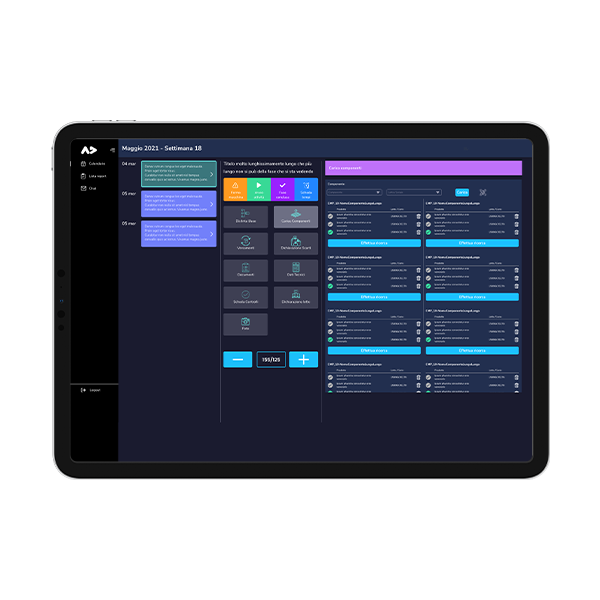
\includegraphics[width=0.8\textwidth]{images/ademes.png}
            \vspace{-20mm}
            \caption[Interfaccia del \textit{software ADeMES}]{Interfaccia del \textit{software ADeMES} \textit{\textbf{Trizeta}}\footnotemark}
        \end{figure}
        \footnotetext{Fonte: \href{https://trizeta.com/ade-mes/}{https://trizeta.com}}
    \item \textbf{Creazione di nuovi prodotti}: in base alle stesse motivazioni espresse al punto precedente, è possibile che la risposta alle nuove esigenze della clientela non sia possibile direttamente all'interno dei prodotti già esistenti (per separazione di ambito o
        per non compromettere la mantenibilità dei prodotti esistenti): in questo caso, concordando lo \glslink{tech-stack}{\textit{stack} tecnologico} da usare, lo \textit{stagista} può implementare un prodotto prototipale \textit{ex-novo} in base alle indicazioni ricevute;
    \item \textbf{Valutazione delle competenze} del tirocinante: il periodo di tirocinio è occasione di introduzione del tirocinante nel contesto aziendale e, per quanto riguarda la mia esperienza, formazione sulla visione aziendale, sui processi in atto, sulle tecnologie utilizzate
        e sulle abilità richieste per l'esecuzione delle attività lavorative; l'azienda ospitante fornisce quindi una formazione di base e valuta quali sono le reazioni agli stimoli (lavorativi e non) in funzione dell'inserimento del tirocinante nel \textit{team} aziendale, data la formazione ricevuta.
        \begin{figure}[H]
            \centering
            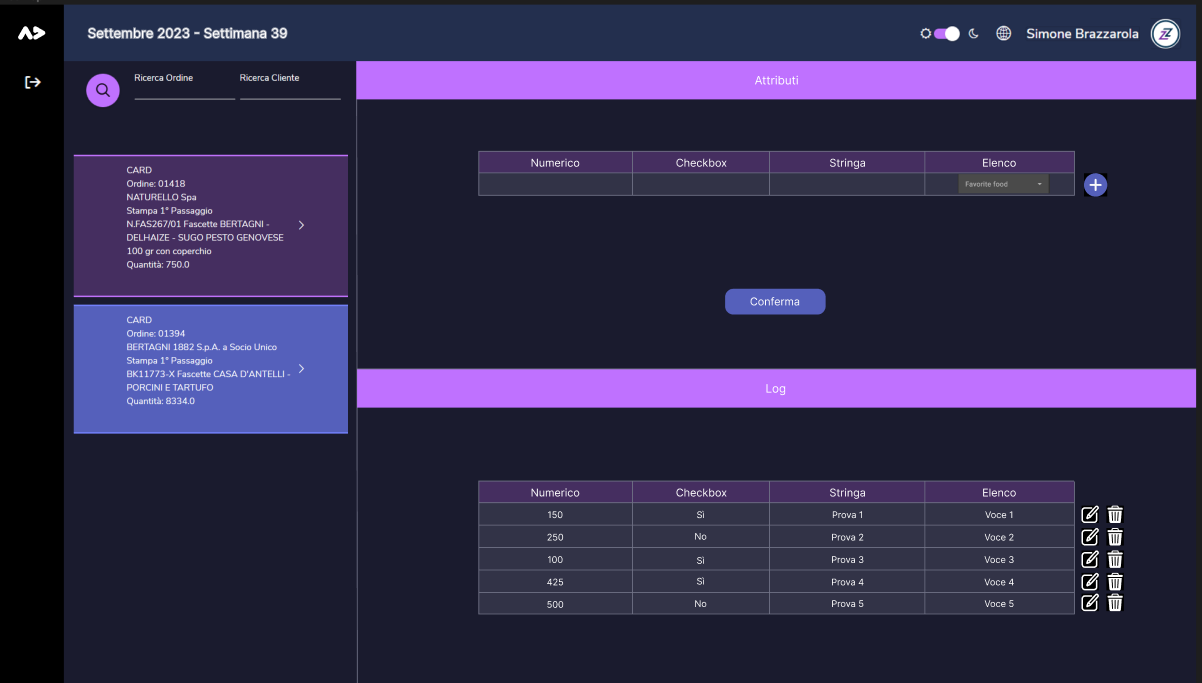
\includegraphics[width=0.8\textwidth]{images/dashboard.png}
            \caption[Interfaccia del prodotto \textit{ADeQA}]{Interfaccia del prodotto \textit{ADeQA}, oggetto del tirocinio}
        \end{figure}
\end{itemize}
\section{Problematiche poste in essere}

% In questa sezione descriverò quali problemi, a livello macroscopico, il prodotto software da me sviluppato ha consentito di superare.
Scopo delle attività di \textit{stage} è la creazione di una \glslink*{pwag}{\textit{progressive web app}} per la raccolta di dati relativi al controllo della qualità delle linee produttive di aziende manifatturiere.
Ogni linea produttiva è costituita da un insieme di "fasi" di lavorazione: ogni fase di lavorazione è considerabile come una \textit{black-box}\footnote{\gls{black-box}} di cui si conoscono gli \textit{input} (materia prima o semilavorati in ingresso)
e gli \textit{output} (semilavorati o prodotti finiti).
\begin{figure}[H]
    \centering
    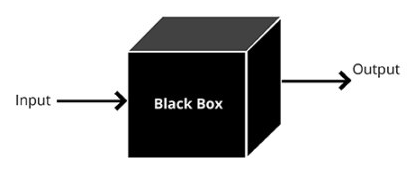
\includegraphics[width=0.6\textwidth]{images/black-box.png}
    \caption[Schema sintesi del concetto di \textit{black-box}]{Schema sintesi del concetto di \textit{black-box}\footnotemark}
\end{figure}
\footnotetext{Fonte: \href{https://www.quora.com/Machine-learning-classifier-is-a-black-box-Why-does-everyone-still-use-it-1}{https://www.quora.com}}
Ogni fase è associata a un insieme di caratteristiche (dette "attributi") relative ai prodotti in uscita dalla stessa: esse sono di interesse per comprendere se la lavorazione ha prodotto articoli utilizzabili nelle fasi successive / nello stoccaggio degli stessi o meno. \\
Non è noto a priori il numero nè il tipo di attributi associati a una determinata fase di lavorazione: sono tutte informazioni ottenibili tramite l'utilizzo di servizi \textit{backend}\footnote{\gls{backend}} (relativi alla struttura ed alla logica di persistenza) esposti dal tutor aziendale con una
serie di \textit{API\footnote{\gls{apig}} REST\footnote{\gls{restg}}} (astrazioni che consentono di eseguire operazioni sui dati di dominio in una architettura \textit{client - server}). \\
L'obiettivo del prodotto è consentire all'utente (operatore in linea di produzione) di inserire, modificare, eliminare e visualizzare dati di controllo qualità per le fasi desiderate (in gergo tecnico, eseguire le operazioni \textit{CRUD}, ovvero \textit{"Create", "Read", "Update" e"Delete"}, sui dati di qualità).

\section{Obiettivi}

Si farà riferimento ai requisiti secondo le seguenti notazioni:
\begin{itemize}
    \item \textbf{O} per i requisiti obbligatori, vincolanti in quanto obiettivo primario richiesto dal committente;
    \item \textbf{D} per i requisiti desiderabili, non vincolanti o strettamente necessari, ma dal riconoscibile valore aggiunto;
    \item \textbf{F} per i requisiti facoltativi, rappresentanti valore aggiunto non strettamente competitivo.
\end{itemize}

Le sigle precedentemente indicate saranno seguite da una coppia sequenziale di numeri, identificativo del requisito.
Di seguito, la lista degli obiettivi di tirocinio:
\begin{itemize}
    \item \textbf{Obbligatori}
        \begin{itemize}
            \item \textbf{O01}: comprensione dei requisiti utente da soddisfare;
            \item \textbf{O02}: studio dell'interfaccia dell'applicazione \textit{ADeMES}, che verrà integrata con il prodotto da sviluppare durante il tirocinio;
            \item \textbf{O03}: acquisizione dela sufficiente dimestichezza con i concetti di base del \textit{framework Angular};
            \item \textbf{O04}: progettazione dell'interfaccia grafica in base allo stile dell'interfaccia dell'applicazione \textit{ADeMES};
            \item \textbf{O05}: sviluppo di una versione di base dell'applicazione \textit{web} che consenta di eseguire le operazioni \textit{CRUD} sui dati di qualità;  
            \item \textbf{O06}: \textit{live demo} della web application in un ambiente simulato;
            \item \textbf{O07}: studio e scelta (motivata) della tecnologia per la fruizione dell'applicazione in lingua inglese.
        \end{itemize}
    \item \textbf{Desiderabili}
        \begin{itemize}
            \item \textbf{D01}: ottimizzazione dei servizi \glslink{restg}{REST} esposti.
        \end{itemize}
    \item \textbf{Facoltativi}
        \begin{itemize}
            \item \textbf{F01}: ottimizzazione dell'esperienza utente per compatibilità con \textit{ADeMES};
            \item \textbf{F02}: ottimizzazione dell'interfaccia grafica, per rendere quanto più simile il prodotto a \textit{ADeMES};
            \item \textbf{F03}: possibilità di fruizione dell'applicazione in lingua spagnola.
        \end{itemize}
\end{itemize}



\section{Vincoli}

% In questa sezione descriverò (entrando nei particolari, rispetto alla sezione precedente) le condizioni imposte ed i risultati prefissati.
Il progetto si focalizza sullo sviluppo di codice prettamente \textit{front-end}\footnote{\gls{frontend}} e questo aspetto caratterizza le condizioni imposte per lo svolgimento del lavoro e le aspettative sul risultato:
\begin{itemize}
    \item Il prodotto deve essere sviluppato usando il \textit{framework Angular} alla versione 16;
    \item Il prodotto deve essere una \glslink{pwa}{PWA};
    \item Il prodotto deve essere utilizzabile dagli operatori di linea produttiva tramite dispositivi mobili (obbligatoriamente tramite \textit{tablet}, facoltativamente tramite \textit{smartphone});
    \item Il prodotto deve poter essere eseguibile in modalità \textit{standalone}\footnote{\gls{standalone}} e deve potersi integrare nel software \textit{ADeMES} mediante un elemento \texttt{<iframe>} \textit{HTML}.
\end{itemize}

\section{Pianificazione}
La pianificazione delle attività, redatta anticipatamente rispetto all'inizio del progetto e disponibile di seguito, è stata rispettata per la maggior parte del tempo: solamente l'interfacciamento coi servizi \glslink{rest}{REST}
di scrittura dati è avvenuto in ritardo, data l'assenza temporanea degli stessi. \\
Di seguito, la suddivisione delle attività pianificate con base settimanale:

\begin{itemize}
    \item \textbf{Prima Settimana (40 ore)}
    \begin{itemize}
        \item Incontro con persone coinvolte nel progetto per discutere i requisiti e le richieste relativamente al sistema da sviluppare;
        \item Verifica credenziali e strumenti di lavoro assegnati;
        \item Presa visione dell’infrastruttura esistente;
        \item Formazione sulle tecnologie adottate.
    \end{itemize}
    \item \textbf{Seconda Settimana - (40 ore)} 
    \begin{itemize}
        \item Analisi e mappatura dei servizi \glslink{rest}{REST} esistenti;
        \item Documentazione dell'analisi dei servizi \glslink{rest}{REST} esistenti.
    \end{itemize}
    \item \textbf{Terza Settimana - (40 ore)} 
    \begin{itemize}
        \item Analisi interfaccia/esperienza utente della \textit{web application};
        \item Documentazione dell'analisi dell'interfaccia della \textit{web application};
        \item Preparazione di un prototipo dimostrativo.
    \end{itemize}
    \item \textbf{Quarta Settimana - (40 ore)} 
    \begin{itemize}
        \item Scelta della tecnologia e del \textit{framework} da utilizzare;
        \item Conclusione della documentazione di analisi;
        \item Documentazione delle scelte progettuali;
        \item Predisposizione infrastruttura della \textit{web application}.
    \end{itemize}
    \item \textbf{Quinta Settimana - (40 ore)} 
    \begin{itemize}
        \item Documentazione delle scelte progettuali;
        \item Sviluppo \textit{web application} ed interfacciamento con i servizi \glslink{rest}{REST} di lettura dati.
    \end{itemize}
    \item \textbf{Sesta Settimana - (40 ore)} 
    \begin{itemize}
        \item Conclusione della documentazione delle scelte progettuali;
        \item Sviluppo \textit{web application} ed interfacciamento con i servizi \glslink{rest}{REST} di scrittura dati.
    \end{itemize}
    \item \textbf{Settima Settimana - (40 ore)} 
    \begin{itemize}
        \item Collaudo \glslink{pwa}{PWA};
        \item \textit{Test} e correzione degli eventuali errori;
        \item Stesura della documentazione finale.
    \end{itemize}
    \item \textbf{Ottava Settimana - Conclusione (40 ore)} 
    \begin{itemize}
        \item Conclusione del collaudo della \glslink{pwa}{PWA};
        \item Conclusione \textit{test} e correzione degli eventuali errori;
        \item Conclusione della stesura della documentazione finale.
    \end{itemize}
\end{itemize}



\section{Scelta del tirocinio}

In questa sezione descriverò le motivazioni che mi hanno portato a scegliere il progetto di tirocinio curricolare, indicando punti a favore e punti a sfavore a monte della scelta.